\chapter{引言}
在现代计算中，尤其是 GPU 编程中，性能在很大程度上取决于多维数据在内存中如何存储与访问。我们关心的大多数数据——例如图像、视频以及机器学习中的张量——本质上是多维的，而计算机的内存从根本上说是一维的。这意味着，当我们想要加载、存储或以其他方式操纵数据时，需要把数据的多维逻辑坐标映射到一维的物理坐标。这种映射被称为{\bf 布局}（layout），它对于正确而高效地读写内存至关重要。此外，在 GPU 的 SIMT 执行模型下，布局还被用来描述与操纵数据上线程的划分，这对于确保优化的内存访问模式、以及正确调用面向张量核心（tensor core）的专用硬件指令十分重要。

作为一个启发性例子，设我们要把 $4 \times 8$ 矩阵
\[
A = 
\begin{bmatrix}
12.47 & 87.21 & 34.08 & 56.93 & 45.65 &  9.17 & 73.02 & 21.39 \\
64.88 & 30.41 &  1.72 & 88.04 & 92.55 & 17.06 & 50.91 & 68.77 \\
 3.33 & 77.19 & 61.58 & 29.46 & 15.82 & 80.75 & 44.62 & 39.28 \\
91.40 & 26.12 &  6.97 & 53.03 & 58.66 & 33.79 & 11.20 & 70.55
\end{bmatrix}
\]
存入内存。为此，我们需要为 $A$ 的每个元素（entry）指定一个内存地址。做法是：为 $A$ 的第 $(0,0)$ 个元素选定某个地址，并为 $A$ 的其余每个元素指定一个{\bf 偏移}（offset）。一种常见的选择是{\bf 行主序}（row-major）布局\\ 

\begin{centering}

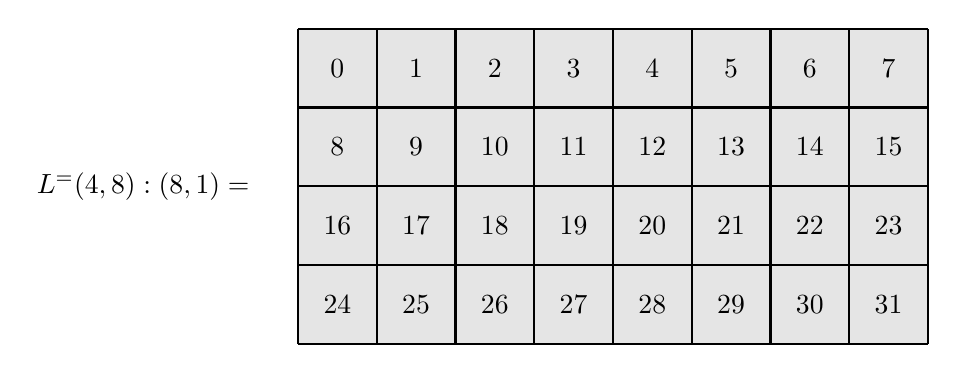
\begin{tikzpicture}[x={(0cm,-1cm)},y={(1cm,0cm)},every node/.style={minimum size=1cm, outer sep=0pt}]

\node[fill=gray!20] at (0,0) {0};
\node[fill=gray!20] at (0,1) {1};
\node[fill=gray!20] at (0,2) {2};
\node[fill=gray!20] at (0,3) {3};
\node[fill=gray!20] at (0,4) {4};
\node[fill=gray!20] at (0,5) {5};
\node[fill=gray!20] at (0,6) {6};
\node[fill=gray!20] at (0,7) {7};
\node[fill=gray!20] at (1,0) {8};
\node[fill=gray!20] at (1,1) {9};
\node[fill=gray!20] at (1,2) {10};
\node[fill=gray!20] at (1,3) {11};
\node[fill=gray!20] at (1,4) {12};
\node[fill=gray!20] at (1,5) {13};
\node[fill=gray!20] at (1,6) {14};
\node[fill=gray!20] at (1,7) {15};
\node[fill=gray!20] at (2,0) {16};
\node[fill=gray!20] at (2,1) {17};
\node[fill=gray!20] at (2,2) {18};
\node[fill=gray!20] at (2,3) {19};
\node[fill=gray!20] at (2,4) {20};
\node[fill=gray!20] at (2,5) {21};
\node[fill=gray!20] at (2,6) {22};
\node[fill=gray!20] at (2,7) {23};
\node[fill=gray!20] at (3,0) {24};
\node[fill=gray!20] at (3,1) {25};
\node[fill=gray!20] at (3,2) {26};
\node[fill=gray!20] at (3,3) {27};
\node[fill=gray!20] at (3,4) {28};
\node[fill=gray!20] at (3,5) {29};
\node[fill=gray!20] at (3,6) {30};
\node[fill=gray!20] at (3,7) {31};
\draw[color=black,thick,shift={(-0.5,-0.5)}] (0,0) grid (4,8);

\node[anchor=east] at (1.5,-1) {$L^\row = (4,8):(8,1) =$};
\end{tikzpicture}

\end{centering}

\bigskip

\noindent 记号 $L^\row = (4,8):(8,1)$ 表示矩阵第 $(i,j)$ 个元素的偏移为
\[
(i,j) \cdot (8,1) = 8i + j. 
\]

\noindent 另一种常见的选择是{\bf 列主序}（column-major）布局 \\

\begin{centering}

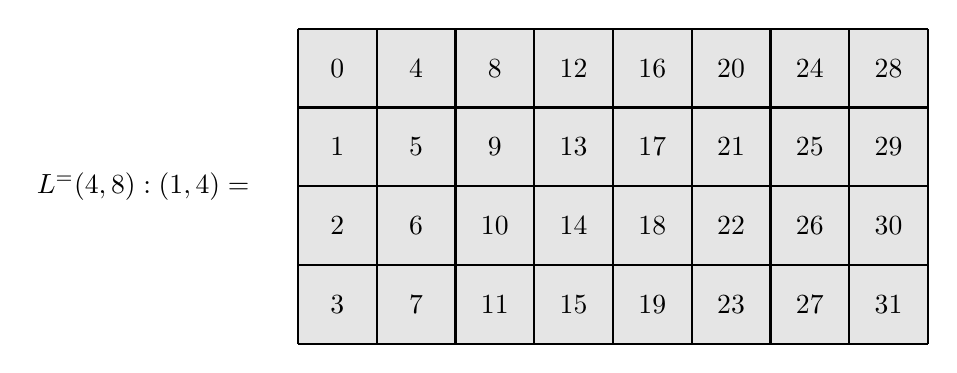
\begin{tikzpicture}[x={(0cm,-1cm)},y={(1cm,0cm)},every node/.style={minimum size=1cm, outer sep=0pt}]

\node[fill=gray!20] at (0,0) {0};
\node[fill=gray!20] at (0,1) {4};
\node[fill=gray!20] at (0,2) {8};
\node[fill=gray!20] at (0,3) {12};
\node[fill=gray!20] at (0,4) {16};
\node[fill=gray!20] at (0,5) {20};
\node[fill=gray!20] at (0,6) {24};
\node[fill=gray!20] at (0,7) {28};
\node[fill=gray!20] at (1,0) {1};
\node[fill=gray!20] at (1,1) {5};
\node[fill=gray!20] at (1,2) {9};
\node[fill=gray!20] at (1,3) {13};
\node[fill=gray!20] at (1,4) {17};
\node[fill=gray!20] at (1,5) {21};
\node[fill=gray!20] at (1,6) {25};
\node[fill=gray!20] at (1,7) {29};
\node[fill=gray!20] at (2,0) {2};
\node[fill=gray!20] at (2,1) {6};
\node[fill=gray!20] at (2,2) {10};
\node[fill=gray!20] at (2,3) {14};
\node[fill=gray!20] at (2,4) {18};
\node[fill=gray!20] at (2,5) {22};
\node[fill=gray!20] at (2,6) {26};
\node[fill=gray!20] at (2,7) {30};
\node[fill=gray!20] at (3,0) {3};
\node[fill=gray!20] at (3,1) {7};
\node[fill=gray!20] at (3,2) {11};
\node[fill=gray!20] at (3,3) {15};
\node[fill=gray!20] at (3,4) {19};
\node[fill=gray!20] at (3,5) {23};
\node[fill=gray!20] at (3,6) {27};
\node[fill=gray!20] at (3,7) {31};
\draw[color=black,thick,shift={(-0.5,-0.5)}] (0,0) grid (4,8);

\node[anchor=east] at (1.5,-1) {$L^\col = (4,8):(1,4) = $};
\end{tikzpicture}

\end{centering} 
\bigskip

\noindent 同样，记号 $L^\col = (4,8):(1,4)$ 表示矩阵第 $(i,j)$ 个元素的偏移为
\[
(i,j) \cdot (1,4) = i + 4j.
\]

\noindent 这些布局极其有用，但并不能满足所有目的。例如，在高性能计算中，人们常常通过如下步骤来计算矩阵乘积 $AB$：
\begin{enumerate}
    \item 把操作数矩阵 $A$ 与 $B$ 划分为若干瓦片（tile），
    \item 计算各瓦片之间的矩阵乘积，以及
    \item 合并这些部分结果以得到完整结果 $AB$。
\end{enumerate}
譬如，我们可以把 $4 \times 8$ 矩阵 $A$ 划分为 $2 \times 2$ 的瓦片，如下所示。
\[
A = \left[\begin{array}{cccc}
\begin{bmatrix}
12.47 & 87.21 \\
64.88 & 30.41 
\end{bmatrix}
&
\begin{bmatrix} 
34.08 & 56.93 \\
1.72 & 88.04 
\end{bmatrix}
&
\begin{bmatrix}
45.65 &  9.17 \\
92.55 & 17.06
\end{bmatrix}
&
\begin{bmatrix} 
73.02 & 21.39 \\
50.91 & 68.77
\end{bmatrix} 
\\[2ex]
\begin{bmatrix}
 3.33 & 77.19 \\
 91.40 & 26.12
\end{bmatrix} 
&
\begin{bmatrix} 
 61.58 & 29.46 \\
6.97 & 53.03 
\end{bmatrix}
&
\begin{bmatrix} 
 15.82 & 80.75 \\
58.66 & 33.79
\end{bmatrix} 
&
\begin{bmatrix} 
 44.62 & 39.28 \\
11.20 & 70.55
\end{bmatrix} 
\end{array}\right]
\]
% \noindent We can consider $A^\tiled$ as a tensor of shape $((2,2),(2,4))$, where 
% \[
% A^\tiled_{(i,j),(k,\ell)} = \begin{matrix}
%     \text{the }(i,j)\text{th entry of} \\
%     \; \;\text{the } (k,\ell)\text{th tile of }A.
% \end{matrix}
% \]

\noindent 现在假设我们想切出 $A$ 的各个瓦片，并设 $A$ 在内存中按列主序格式存放。为此，可以按如下方式手工计算偏移：对第 $(i,j)$ 个瓦片，索引其左上角元素的偏移由 $2i + 8j$ 给出。另一方面，为了更好地组织这一计算，我们可以使用瓦片的{\bf 交错}（interleaved）布局
\\


\begin{centering}

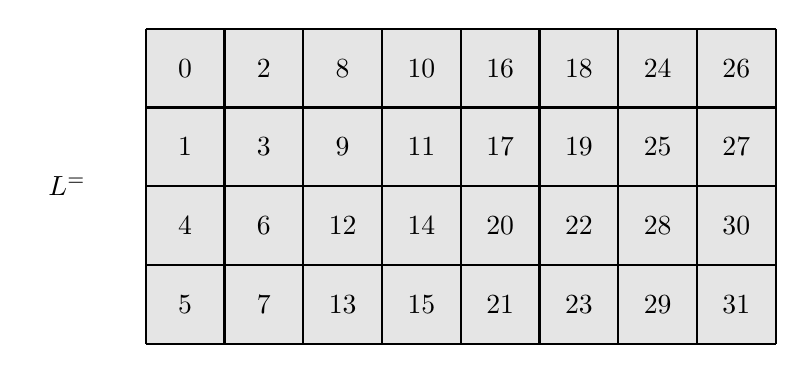
\begin{tikzpicture}[x={(0cm,-1cm)},y={(1cm,0cm)},every node/.style={minimum size=1cm, outer sep=0pt}]

\node[fill=gray!20]       at (0,0) {0};
\node[fill=gray!20]       at (0,1) {2};
\node[fill=gray!20]      at (0,2) {8};
\node[fill=gray!20]      at (0,3) {10};
\node[fill=gray!20]  at (0,4) {16};
\node[fill=gray!20]  at (0,5) {18};
\node[fill=gray!20]        at (0,6) {24};
\node[fill=gray!20]        at (0,7) {26};

\node[fill=gray!20]       at (1,0) {1};
\node[fill=gray!20]       at (1,1) {3};
\node[fill=gray!20]      at (1,2) {9};
\node[fill=gray!20]      at (1,3) {11};
\node[fill=gray!20]  at (1,4) {17};
\node[fill=gray!20]  at (1,5) {19};
\node[fill=gray!20]        at (1,6) {25};
\node[fill=gray!20]        at (1,7) {27};

\node[fill=gray!20]       at (2,0) {4};
\node[fill=gray!20]       at (2,1) {6};
\node[fill=gray!20]      at (2,2) {12};
\node[fill=gray!20]      at (2,3) {14};
\node[fill=gray!20]  at (2,4) {20};
\node[fill=gray!20]  at (2,5) {22};
\node[fill=gray!20]        at (2,6) {28};
\node[fill=gray!20]        at (2,7) {30};

\node[fill=gray!20]       at (3,0) {5};
\node[fill=gray!20]       at (3,1) {7};
\node[fill=gray!20]      at (3,2) {13};
\node[fill=gray!20]      at (3,3) {15};
\node[fill=gray!20]  at (3,4) {21};
\node[fill=gray!20]  at (3,5) {23};
\node[fill=gray!20]        at (3,6) {29};
\node[fill=gray!20]        at (3,7) {31};
\draw[color=black,thick,shift={(-0.5,-0.5)}] (0,0) grid (4,8);

\node[anchor=east] at (1.5,-1) {$L^\tiled =$};

% \node at (0,-1) {\Large{\texttt{0}}};
% \node at (1,-1) {\Large{\texttt{1}}};
% \node at (2,-1) {\Large{\texttt{2}}};
% \node at (3,-1) {\Large{\texttt{3}}};
% \node at (-1,0) {\Large{\texttt{0}}};
% \node at (-1,1) {\Large{\texttt{1}}};
% \node at (-1,2) {\Large{\texttt{2}}};
% \node at (-1,3) {\Large{\texttt{3}}};
% \node at (-1,4) {\Large{\texttt{4}}};
% \node at (-1,5) {\Large{\texttt{5}}};
% \node at (-1,6) {\Large{\texttt{6}}};
% \node at (-1,7) {\Large{\texttt{7}}};
\end{tikzpicture}

\end{centering}

\bigskip

\noindent 其中列由 $A$ 的瓦片给出，行由瓦片形状内的坐标给出。这里我们用{\bf 余字典序}（colexicographic ordering）来线性地枚举瓦片以及瓦片内的坐标，因此布局 $L^\tiled$ 的顶层形状为 $(4, 8)$。

然而，请注意，$L^\tiled$ 所呈现的交错模式意味着，对任何步长 $a,b$，它都不能表示为布局 $(4,8):(a,b)$。作为替代，我们可以把形状 $(4,8)$ 的各模式分解因式，并定义
\[ L^\tiled = ((2,2),(2,4)):((1,4),(2,8)). \]

\noindent 这样，前面的偏移计算 $2i + 8j$ 就体现为在坐标 $(0, (i,j))$ 上对 $L^\tiled$ 求值，而瓦片布局本身则由第一个模式给出。于是，在为 $A$ 赋予布局 $L^\tiled$ 而得到 $A^\tiled$ 之后，我们就可以把 $A$ 的第 $(i,j)$ 个瓦片取为切片

\[ A_{i,j} = A^\tiled(\; \rule{.7em}{0.4pt} \; , (i,j)). \]

CUTLASS 中发展的一个关键思想是：像 $L^\tiled$ 这样有用但更复杂的辅助布局，可以通过某些基本运算从更简单的布局系统地推导出来。就 $L^\tiled$ 而言，所涉及的运算称为{\bf 逻辑切分}（logical division）。若记
\\

\begin{centering}

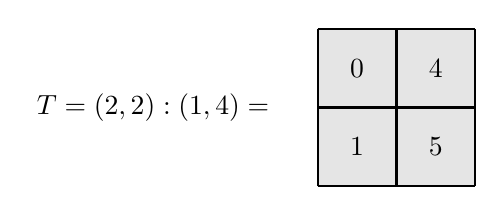
\begin{tikzpicture}[x={(0cm,-1cm)},y={(1cm,0cm)},every node/.style={minimum size=1cm, outer sep=0pt}]
\node[fill=gray!20]       at (0,0) {0};
\node[fill=gray!20]       at (1,0) {1};
\node[fill=gray!20]      at (0,1) {4};
\node[fill=gray!20]      at (1,1) {5};
\draw[color=black,thick,shift={(-0.5,-0.5)}] (0,0) grid (2,2);

\node[anchor=east] at (0.5,-1) {$T = (2,2):(1,4) =$};
\end{tikzpicture}

\end{centering}

\bigskip

\noindent 为瓦片布局，则 $L^\tiled$ 就是逻辑切分

\[
L^\tiled = L^\col \oslash T
\]
如下图所示。\\

\begin{centering}
\begin{tikzpicture}[x={(0cm,-1cm)},y={(1cm,0cm)},every node/.style={minimum size=1cm, outer sep=0pt}]

\node[fill=colorx1!60] at (0,0) {0};
\node[fill=colorx1!60] at (0,1) {4};
\node[fill=colorx3!60] at (0,2) {8};
\node[fill=colorx3!60] at (0,3) {12};
\node[fill=colorx5!60] at (0,4) {16};
\node[fill=colorx5!60] at (0,5) {20};
\node[fill=colorx7!60] at (0,6) {24};
\node[fill=colorx7!60] at (0,7) {28};
\node[fill=colorx1!60] at (1,0) {1};
\node[fill=colorx1!60] at (1,1) {5};
\node[fill=colorx3!60] at (1,2) {9};
\node[fill=colorx3!60] at (1,3) {13};
\node[fill=colorx5!60] at (1,4) {17};
\node[fill=colorx5!60] at (1,5) {21};
\node[fill=colorx7!60] at (1,6) {25};
\node[fill=colorx7!60] at (1,7) {29};
\node[fill=colorx2!60] at (2,0) {2};
\node[fill=colorx2!60] at (2,1) {6};
\node[fill=colorx4!60] at (2,2) {10};
\node[fill=colorx4!60] at (2,3) {14};
\node[fill=colorx6!60] at (2,4) {18};
\node[fill=colorx6!60] at (2,5) {22};
\node[fill=colorx8!60] at (2,6) {26};
\node[fill=colorx8!60] at (2,7) {30};
\node[fill=colorx2!60] at (3,0) {3};
\node[fill=colorx2!60] at (3,1) {7};
\node[fill=colorx4!60] at (3,2) {11};
\node[fill=colorx4!60] at (3,3) {15};
\node[fill=colorx6!60] at (3,4) {19};
\node[fill=colorx6!60] at (3,5) {23};
\node[fill=colorx8!60] at (3,6) {27};
\node[fill=colorx8!60] at (3,7) {31};
\draw[color=black,thick,shift={(-0.5,-0.5)}] (0,0) grid (4,8);

\node[anchor = east] at (1.5,-1) {$L^\col = $ };
\node[anchor = east] at (1.5,9.5) {$T = $};

\node[fill=gray!5] at (1,10) {0};
\node[fill=gray!20] at (2,10) {1};
\node[fill=gray!40] at (1,11) {4};
\node[fill=gray!60] at (2,11) {5};
\draw[color=black,thick,shift={(-0.5,-0.5)}] (1,10) grid (3,12);
\end{tikzpicture}

\end{centering}

\vspace{0.2in}

\begin{centering}
\begin{tikzpicture}[x={(0cm,-1cm)},y={(1cm,0cm)},every node/.style={minimum size=1cm, outer sep=0pt}]

\node[fill=colorx1!10]       at (0,0) {0};
\node[fill=colorx2!10]       at (0,1) {2};
\node[fill=colorx3!10]      at (0,2) {8};
\node[fill=colorx4!10]      at (0,3) {10};
\node[fill=colorx5!10]  at (0,4) {16};
\node[fill=colorx6!10]  at (0,5) {18};
\node[fill=colorx7!10]        at (0,6) {24};
\node[fill=colorx8!10]        at (0,7) {26};

\node[fill=colorx1!25]       at (1,0) {1};
\node[fill=colorx2!25]       at (1,1) {3};
\node[fill=colorx3!25]      at (1,2) {9};
\node[fill=colorx4!25]      at (1,3) {11};
\node[fill=colorx5!25]  at (1,4) {17};
\node[fill=colorx6!25]  at (1,5) {19};
\node[fill=colorx7!25]        at (1,6) {25};
\node[fill=colorx8!25]        at (1,7) {27};

\node[fill=colorx1!40]       at (2,0) {4};
\node[fill=colorx2!40]       at (2,1) {6};
\node[fill=colorx3!40]      at (2,2) {12};
\node[fill=colorx4!40]      at (2,3) {14};
\node[fill=colorx5!40]  at (2,4) {20};
\node[fill=colorx6!40]  at (2,5) {22};
\node[fill=colorx7!40]        at (2,6) {28};
\node[fill=colorx8!40]        at (2,7) {30};

\node[fill=colorx1!60]       at (3,0) {5};
\node[fill=colorx2!60]       at (3,1) {7};
\node[fill=colorx3!60]      at (3,2) {13};
\node[fill=colorx4!60]      at (3,3) {15};
\node[fill=colorx5!60]  at (3,4) {21};
\node[fill=colorx6!60]  at (3,5) {23};
\node[fill=colorx7!60]       at (3,6) {29};
\node[fill=colorx8!60]       at (3,7) {31};
\draw[color=black,thick,shift={(-0.5,-0.5)}] (0,0) grid (4,8);

\node[anchor=east] at (1.5,-1) {$ L^\col \oslash T = $};

% \node at (0,-1) {\Large{\texttt{0}}};
% \node at (1,-1) {\Large{\texttt{1}}};
% \node at (2,-1) {\Large{\texttt{2}}};
% \node at (3,-1) {\Large{\texttt{3}}};
% \node at (-1,0) {\Large{\texttt{0}}};
% \node at (-1,1) {\Large{\texttt{1}}};
% \node at (-1,2) {\Large{\texttt{2}}};
% \node at (-1,3) {\Large{\texttt{3}}};
% \node at (-1,4) {\Large{\texttt{4}}};
% \node at (-1,5) {\Large{\texttt{5}}};
% \node at (-1,6) {\Large{\texttt{6}}};
% \node at (-1,7) {\Large{\texttt{7}}};
\end{tikzpicture}

\end{centering}

\bigskip

除逻辑切分之外，其他基本的布局运算还包括{\bf 逻辑乘积}（logical product）、{\bf 补}（complement），以及最重要的{\bf 复合}（composition）。这些布局运算是 CUTLASS 的支柱，深入理解它们的行为有助于编写正确且高性能的代码。然而，这些运算的定义与构造相当精妙。例如，布局 $A$ 与 $B$ 的复合 $B \circ A$ 只有在 $A$ 与 $B$ 满足某些整除性约束时才是良定义（well-defined）的，CUTLASS 会在底层检查这些约束。特别地，两个布局何时可复合、以及应如何解释它们的复合，并不总是显然的。

% To support these tasks, NVIDIA's CUTLASS library provides a powerful toolkit for working with layouts. The core abstraction of the CUTLASS library is the {\bf CuTe layout}, or simply {\bf layout}, which specifies a logical-to-physical coordinate transformation (\cite{cutedsldocumentation}, \cite{cutedocumentation}). Throughout this work, we include code snippets written in NVIDIA’s CuTe DSL, a Python-based implementation of CuTe, which we refer to simply as $\texttt{cute}$. CuTe layouts and the operations which they support abstract away the complexity of layout management, allowing programmers to work with high-dimensional structures efficiently and intuitively. The power of layouts comes from the vast collection of operations they support.

% Given the subtlety of these operations, there is a clear need for a more accessible and mathematically grounded treatment of layouts.

% TODO: Get Cris Cecka consent or not to mention his forthcoming work.
% Mathematically, the theory of {\bf categories} and {\bf operads} provides a convenient language and set of standard mathematical tools for describing and reasoning about algebraic structures with a notion of composition. In this work, we will adopt a categorical perspective in order to develop one possible mathematical framework for CuTe layouts, although knowledge of category theory or operads isn't a strict prerequisite to read this work. We mention here that another framework has been developed in forthcoming work by Cris Cecka, the original author of CuTe, and the reader may wish to compare his perspective with ours.

\section{主要结果综述}

本文的主要思想是：通过把注意力限制在{\bf 可处理布局}（tractable layout）上——其元素满足一个简单的整除性条件（见定义 \ref{definitionoftractablelayouts}）——我们可以为布局的操纵发展出一套直观而强大的数学框架。可处理布局几乎涵盖了实践中会遇到的所有布局，例如
\begin{itemize}
\item {\it 行主序}与{\it 列主序}布局，它们无处不在；
\item {\it 紧凑}（compact）布局，它们把数据存储在连续的内存地址中；
\item {\it 投影}（projection）布局，它们广播数据的多个副本；以及
\item {\it 膨胀}（dilation）布局，它们支持带填充的加载与存储。
\end{itemize}
若 $L$ 是可处理布局，则我们可以用{\bf 图表}（diagram）来表示 $L$。例如，布局 $L^\row$、$L^\col$ 与 $L^\tiled$ 由下列图表表示。

\[\begin{tikzcd}[row sep = 1, column sep = 12]
  & & & &  & & 8 \ar[drr,mapsto] & & 4 \\
 (4,8):(8,1) & & \leftrightsquigarrow & &   & & 4 \ar[urr,mapsto] & & 8 \\
  & & & &  & &   & &  \\
 & & & &   & &   & &   \\[2em]
 & & & &   & &   & &  \\
 & & & &   & & 8 \ar[rr,mapsto] & & 8  \\
(4,8):(1,4)& & \leftrightsquigarrow& &   & & 4 \ar[rr,mapsto] & & 4  \\
  & & & &  & &   & &    \\
 & & & &   & &   & &   \\[2em]
 & & & &   & &   & &    \\
 & & & &  & & 4 \ar[rr,mapsto] & & 4  \\
& & & & 8 \ar[rr,-] \ar[urr,-] & & 2 \ar[drr,mapsto] & & 2 & & & & \\
 ((2,2),(2,4)):((1,4),(2,8)) & & \leftrightsquigarrow & &   & & 2 \ar[urr,mapsto] & & 2 \\
& & & & 4 \ar[urr,-] \ar[rr,-]  & & 2 \ar[rr,mapsto] & & 2  \\
& & & &   & &   & &   \\
\end{tikzcd}\]
% \[\begin{tikzcd}[row sep = 1, column sep = 8]
% & & & & & & & &  & & \\
% & & & & & & & & & & 4\\
%     (4,4) \ar[rrrr,"f"] \ar[rrrr,swap,"(1{,}3)"] & & & & (4,2,4)  & & \rightsquigarrow & & 4 \ar[urr,mapsto] & & 2\\
%     & & & & & & & & 4 \ar[rr,mapsto] & & 4\\
%     & & & & & & & &  & f &\\
% & & & & & & & & & & \\[2em]
% & & & & & & & & 2 \ar[drr,mapsto] & & 2\\
%     (2,2,2) \ar[rrrr,"g"] \ar[rrrr,swap,"(1{,}3{,}2)"] & & & & (2,2,2)  & & \rightsquigarrow & & 2 \ar[urr,mapsto] & & 2\\
%     & & & & & & & & 2 \ar[rr,mapsto] & & 2\\
%     & & & & & & & &  & g &
% & & & & & & & & & & \\[2em]
% & & & & & & & & 4 & & \\
% & & & & & & & & 4 \ar[drr,mapsto] & & \\
% & & & & & & & & 4 & & 4\\
%     (16,(4,4),(4,4)) \ar[rrrr,"h"] \ar[rrrr,swap,"(1{,}2{,}*{,}3{,}*)"] & & & & (16,4,4)  & & \rightsquigarrow & & 4 \ar[rr,mapsto] & & 4\\
%     & & & & & & & & 16 \ar[rr,mapsto] & & 16\\
%     & & & & & & & &  & h &
% \end{tikzcd}\]

\noindent 这些图表可以解释为某个{\bf 范畴}（category）中的态射（morphism）。这使我们得以借助{\bf 范畴论}（category theory）的力量来描述布局及其运算。\footnote{对于不熟悉这一学科的读者，我们在附录 \ref{categorytheoryappendix} 中提供了范畴论入门。}

更确切地说，我们定义一个范畴 $\catstyle{Nest}$，其对象（object）是正整数的嵌套元组（nested tuple），其态射 $f:S \to T$ 对应于如上那种图表（详见定义 \ref{definitionofTuple} 与定义 \ref{definitionofNest}）。若 $L$ 是{\bf 非退化}（non-degenerate）的可处理布局（见定义 \ref{definitionofnondegeneratelayout}），则存在一个本质唯一的 $\catstyle{Nest}$-态射 $f$ 编码 $L$，正如下面的对应定理所展示的那样。
% An object of $\catstyle{Nest}$ is a nested tuples of positive integers, and a morphism $f:S \to T$ in $\catstyle{Nest}$ associates entries of $S$ to entries of $T$ (see Definition \ref{definitionofTuple} and Definition \ref{definitionofNest}). If $f:S \to T$ is a nested tuple morphism, then $f$ encodes a tractable layout $L_f$. The shape of $L_f$ is $S$, and the stride of $L_f$ is a nested tuple whose entries are certain prefix products of $T$ (See Construction \ref{layoutfromnestedtuplemorphism}). For example, the layouts encoded by the morphisms $f$, $g$, and $h$ above are
% \begin{align*}
%     L_f & = (4,4):(1,8)\\
%     L_g & = (2,2,2):(1,4,2)\\
%     L_h & = (16,(4,4),(4,4)): (1,(16,0),(64,0)).
% \end{align*}

 % Conversely, if $L$ is a tractable layout, then there exists a nested tuple morphism $f_L$ which encodes $L$. The nested tuple morphism which encodes $L$ is not unique. However, we introduce a notion of {\it standard form} for nested tuple morphisms (Definition \ref{definitionofnestedstandardform}), and prove the following correspondence theorem.
\begin{mainthm}(参见 \ref{nestedonetoonecorrespondence})
存在一一对应
    \[ \begin{tikzcd} 
    \begin{Bmatrix}
    \text{非退化}\\
        \text{可处理布局}
    \end{Bmatrix} 
    \ar[r] & \ar[l] 
        \begin{Bmatrix}
        \text{非退化}\\
        \catstyle{Nest}\text{-态射}\\
        \text{（标准形式）}
    \end{Bmatrix}
    \end{tikzcd} 
    \]
\end{mainthm}

诸如复合、逻辑切分与逻辑乘积这样的布局运算，都可以在范畴 $\catstyle{Nest}$ 中得到自然的解释。若
\[
\begin{tikzcd}
    S \ar[r,"f"]  & T \ar[r,"g"]  & U
\end{tikzcd}
\]
是 $\catstyle{Nest}$-态射，则我们可以通过把相应的图表粘合在一起来构成复合
\[\begin{tikzcd}
S \ar[r,"g \circ f"] &  U
\end{tikzcd} \]
例如，
% \[\begin{tikzcd}
% (2,2) \ar[rr,"f"] \ar[rr,swap,"(2{,}1)"] & & (2,2) \ar[rr,"g"] \ar[rr,swap,"(2{,}3)"] & & (5,(2,2))
% \end{tikzcd}\]
% is 
% \[\begin{tikzcd}
% (2,2) \ar[rr,"g \circ f"] \ar[rr,swap,"(3{,}2)"] & &  (5,(2,2))
% \end{tikzcd}\]
% as depicted below.
\[ \begin{tikzcd}[row sep = 1, column sep = 8]
 & &   & & 2 & & & & & & 2\\
2 \ar[drr,mapsto]  & & 2 \ar[urr,mapsto] & & 2 & & \rightsquigarrow & & 2 \ar[rr,mapsto]  & & 2\\
2 \ar[urr,mapsto] & & 2 \ar[urr,mapsto] & & 5 & & & & 2 \ar[uurr,mapsto] & & 5\\
 & f & & g & & & & & & \mathclap{g \circ f} & 
\end{tikzcd}\]
我们证明 $\catstyle{Nest}$ 中的复合与布局复合相容。
\begin{mainthm}(参见 \ref{compatibilityofcompositioninD}) 若 $f$ 与 $g$ 是非退化的、可复合的 $\catstyle{Nest}$-态射，则
\[
L_{g \circ f} = L_g \circ L_f.
\]
\end{mainthm}
% For example, if $f$ and $g$ are the morphisms above, then 
% \begin{align*}
%     L_f & =(2,2):(2,1) \\
%     L_g & = (2,2):(5,10)\\
%     L_{g \circ f} & = (2,2):(10,5)\\
%     L_g \circ L_f& = (2,2):(10,5).
% \end{align*}

我们可以通过折叠相邻的箭头来合并（coalesce）$\catstyle{Nest}$-态射 $f$。例如，
% on nested tuple morphisms.
% For example if $f$ is the morphism 
% \[
% \begin{tikzcd} 
% ((2,2),(10,10)) \ar[rr,"f"] \ar[rr,swap,"(1{,}2{,}4{,}5)"] & & (2,2,2,10,10)
% \end{tikzcd}
% \]
% then $\coalesce(f)$ is the morphism 
% \[
% \begin{tikzcd} 
% (4,100) \ar[rr,"\coalesce(f)"] \ar[rr,swap,"(1{,}3)"] & & (4,2,100)
% \end{tikzcd}
% \]
% as depicted below.
\[\begin{tikzcd}[row sep = 1, column sep = 8]
 & & 10 & & & & & & \\
 10 \ar[urr,mapsto] & & 10 & & & & & & \\
 10 \ar[urr,mapsto] & & 2 & & & & & & 100\\
 2 \ar[rr,mapsto] & & 2 & & \rightsquigarrow & & 100 \ar[urr,mapsto] & & 2\\
 2 \ar[rr,mapsto] & & 2 & & & & 4 \ar[rr,mapsto] & & 4\\
    & f & & & & & & \mathclap{\coalesce(f)} & 
\end{tikzcd}\]
我们证明该运算与布局的合并运算相容。
\begin{mainthm}(参见 \ref{coalesceagreement}) 若 $f$ 是 $\catstyle{Nest}$-态射，则
\[
L_{\coalesce(f)} = \coalesce(L_f).
\]
\end{mainthm}
% For example, if $f$ is the morphism above, then 
% \begin{align*}
%     L_f & = ((2,2),(10,10)):((1,2),(8,80))\\
%     L_{\coalesce(f)} & = (4,100):(1,8)\\
%     \coalesce(L_f) & = (4,100):(1,8).
% \end{align*}

$\catstyle{Nest}$-态射 $f$ 的补是未被 $f$ 命中的元素所构成的包含映射（inclusion）。例如，
% if $f$ is the morphism 
% \[
% \begin{tikzcd} 
% (2,2) \ar[rr,"f"] \ar[rr,swap,"(1{,}3)"] & & (2,5,2,5)
% \end{tikzcd}
% \]
% then $f^c$ is the morphism 
% \[
% \begin{tikzcd} 
% (5,5) \ar[rr,"f^c"] \ar[rr,swap,"(2{,}4)"] & & (2,5,2,5)
% \end{tikzcd}
% \]
% as depicted below.
\[\begin{tikzcd}[row sep = 1, column sep = 8]
 & & 5 & & & & & & 5\\
 & & 2 & & & & & & 2\\
 2 \ar[urr,mapsto] & & 5 & & \rightsquigarrow &  & 5 \ar[uurr,mapsto] & & 5\\
 2 \ar[rr,mapsto] & & 2 & & & &  5 \ar[urr,mapsto]  & & 2\\
    & f & & & & & &  f^c & 
\end{tikzcd}\]
我们证明 $\catstyle{Nest}$ 中的补与布局的补相容。
\begin{mainthm}(参见 \ref{coalescedlayoutoftuplemorphismcomplement}) 若 $f:S \to T$ 是单射的 $\catstyle{Nest}$-态射且 $N = \size(T)$，则
\[
\coalesce(L_{f^c}) = \comp(L_f,N).
\]
\end{mainthm} 
% For example, if $f$ is the morphism above, then 
% \begin{align*}
% L_f & = (2,2):(1,10)\\
% L_{f^c} & = (5,5):(2,20)\\
% \comp(L_f,100)&  = (5,5):(2,20).
% \end{align*}

我们定义 $\catstyle{Nest}$-态射的整除性，以及当 $g$ 整除 $f$ 时的逻辑切分运算
\[
f,g \mapsto f \oslash g
\]
例如，
% if $f$ and $g$ are the morphisms 
% \[\begin{tikzcd}
%     ((4,8),(4,8)) \ar[rr,"f"] \ar[rr,swap,"(1{,}2{,}3{,}4)"] & & ((4,8),(4,8))\\
%     (4,4) \ar[rr,"g"] \ar[rr,swap,"(1{,}3)"] & & ((4,8),(4,8))
% \end{tikzcd}\]
% then $g$ divides $f$, and $f \oslash g$ is the morphism 
% \[\begin{tikzcd}
%     ((4,4),(8,8)) \ar[rr,"f\oslash g"] \ar[rr,swap,"(1{,}3{,}2{,}4)"] & & ((4,8),(4,8))
% \end{tikzcd}\]
% as depicted below.
\[\begin{tikzcd}[row sep = 1, column sep = 8]
  & & 8 \ar[rr,mapsto] & & 8 & & & & & &  8 \ar[rr,mapsto]  & & 8\\
  & & 4 \ar[rr,mapsto] & & 4 & & & & 64 \ar[rr,-] \ar[urr,-]& &  8 \ar[drr,mapsto] & & 4\\
4 \ar[urr,mapsto] & & 8 \ar[rr,mapsto] & & 8 & & \rightsquigarrow & &  & &  4 \ar[urr,mapsto] & & 8\\
4 \ar[rr,mapsto] & & 4 \ar[rr,mapsto] & & 4 & & & & 16 \ar[rr,-] \ar[urr,-]& & 4 \ar[rr,mapsto] & & 4\\
  & g &  & f & & & & & & & & \mathclap{f \oslash g} & 
\end{tikzcd}\]

我们证明 $\catstyle{Nest}$ 中的逻辑切分与布局的逻辑切分相容。
\begin{mainthm}(参见 \ref{coalesceoflogicaldivision}) 若 $f$ 与 $g$ 是非退化 $\catstyle{Nest}$-态射且 $g$ 整除 $f$，则
\[
\coalesce(L_{f \oslash g}) = \coalesce(L_f \oslash L_g).
\]
\end{mainthm}
% For example, if $f$ and $g$ are the morphisms above, then 
% \begin{align*}
%     L_f & = (4,8,4,8):(1,4,32,128)\\
%     L_g & = (4,4):(1,32)\\
%     L_{f \oslash g} & = ((4,4),(8,8)):((1,32),(4,128))\\
%     L_f \oslash L_g & = ((4,4),(8,8)):((1,32),(4,128)).
% \end{align*}

我们定义 $\catstyle{Nest}$-态射的乘积可许性（product admissibility），以及当 $f$ 与 $g$ 乘积可许时的逻辑乘积运算
\[
f,g \mapsto f \otimes g
\]
例如，
% if $f$ and $g$ are the nested tuple morphisms 
% \[\begin{tikzcd}
%     (2,2) \ar[rr,"f"] \ar[rr,swap,"(1{,}2)"] & & (2,2,5,5)\\
%     (5,5) \ar[rr,"g"] \ar[rr,swap,"(2{,}1)"] & & (5,5)
% \end{tikzcd}\]
% then $f$ and $g$ are product admissible, and $f \otimes g$ is the morphism 
% \[\begin{tikzcd}
%     ((2,2),(5,5)) \ar[rr,"f\oslash g"] \ar[rr,swap,"(1{,}2{,}4{,}3)"] & & (2,2,5,5)
% \end{tikzcd}\]
% as depicted below.
\[\begin{tikzcd}[row sep = 1, column sep = 8]
  & & 5 & &   & &  & &  & & & & 5 \ar[drr,mapsto] & & 5\\
  & & 5 & &   & & & & & & 25 \ar[rr,-] \ar[urr,-] & & 5 \ar[urr,mapsto] & & 5\\
2  \ar[rr,mapsto] & & 2 & & 5  \ar[drr,mapsto] & & 5 & & \rightsquigarrow & & &  & 2 \ar[rr,mapsto] & & 2\\
2 \ar[rr,mapsto] & & 2 & & 5 \ar[urr,mapsto]  & & 5 & & & & 4 \ar[rr,-] \ar[urr,-] & & 2 \ar[rr,mapsto] & & 2\\
  & f & & &  & g & & & & & & & & \mathclap{f \otimes g} & 
\end{tikzcd}\] 


我们证明 $\catstyle{Nest}$ 中的逻辑乘积与布局的逻辑乘积相容。
\begin{mainthm}(参见 \ref{logicalproductcompatibility}) 若 $f$ 与 $g$ 是非退化 $\catstyle{Nest}$-态射且二者乘积可许，则
\[
L_{f \otimes g} = L_f \otimes L_g.
\]
\end{mainthm}
% For example, if $f$ and $g$ are the morphisms above, then 
% \begin{align*}
%     L_f & = (2,2):(1,2)\\
%     L_g & = (5,5):(5,1) \\
%     L_{f \otimes g} & = ((2,2),(5,5)):((1,2),(20,4))\\
%     L_f \otimes L_g & = ((2,2),(5,5)):((1,2),(20,4))
% \end{align*}

在第 \ref{computationschapter} 章中，我们展示如何用我们的新框架来计算复合、逻辑切分与逻辑乘积等重要布局运算。特别地，我们给出一个计算可处理布局 $A$ 与 $B$ 的复合 $B \circ A$ 的算法（算法 \ref{tractablelayoutcompositionalgorithm}）。略去细节，我们算法的基本思想是：若要计算复合 $B \circ A$，可以用适当选取的 $\catstyle{Nest}$-态射 $f$ 与 $g$ 分别表示 $A$ 与 $B$，把这两个态射复合成 $g \circ f$，再取其编码的布局，从而得到
\[
B \circ A = L_{g \circ f}.
\]
我们用大量例子演示这一算法。

\section{结构安排}

本文的组织结构如下。 

在 \ref{implementationsection} 节中，我们给出布局的 $\texttt{cute}$ 实现的相关细节。我们以模块 $\texttt{tract}$ 的形式提供了范畴 $\catstyle{Nest}$ 的一个 Python 实现，并演示 $\texttt{tract}$ 与 $\texttt{cute}$ 的相容性。我们的 Python 实现可在我们的 git 仓库 \url{https://github.com/ColfaxResearch/layout-categories} 找到。

第 \ref{layoutschapter} 章是关于布局及其代数的全面参考。该章给出布局及其所支持运算的严格定义，并建立这些运算的基本性质。该章富含例子，对一线程序员也可能颇有助益。 

在第 \ref{categorieschapter} 章中，我们提出一个处理可处理布局的新数学框架。特别地，我们把布局及其代数与{\bf 范畴}和 {\bf operad} 的理论联系起来。该章内容具有独立的数学趣味，同时也有实用价值：它为可视化布局以及计算布局的各种运算提供了一个新框架。  

在第 \ref{computationschapter} 章中，我们利用第 \ref{categorieschapter} 章发展的框架，给出一个计算可处理布局 $A$ 与 $B$ 的复合的算法。我们用大量例子演示该复合算法。

\section{相关工作}

虽然本文在性质上是理论性的，但其动机来自 GPU 编程中的实际应用，最著名的当属 CUTLASS。我们强调，这里发展的理论是独立于实现的：它不依赖于在实践中用来实现布局的具体编程语言或运行时系统。尽管如此，在使用具体实现时仍会出现一些实际的考量。例如，CUTLASS 会区分编译期常量（静态变量）与运行时值（动态变量）。这一信息使编译器能够在代码生成期间进行优化。这类与实现相关的细节虽然对性能很重要，但超出了我们数学框架的讨论范围。进一步的讨论见 CuTe 文档 \cite{cutedocumentation}。

我们为布局发展的数学框架与计算机科学和数学的若干领域都有关联。我们简要回顾 GPU 编程及相邻领域的相关工作，以便为我们的贡献提供更完整的背景。

\begin{itemize}
    \item {\bf CUTLASS 的应用。}CUTLASS 的最先进应用包括 FlashAttention \cite{dao2023flashattention2, shah2024flashattention3}、EVT \cite{chen2024evt} 与 SonicMoE \cite{sonic}。对于希望更深入地理解 CUTLASS 与 CuTe 实际应用的读者，我们推荐 NVIDIA~\cite{cecka2024cutlass, sun2025cutlass, thakkar2025cutlass} 与 Colfax Research~\cite{shah2024cutlass_streamk, shah2025cutlass_blackwell_tensor_memory, shah2025cutlass_blackwell_clusters, shah2025cutlass_blackwell_subbyte} 关于用这些库进行 GPU 编程的系列综合教程。
    \item {\bf 数据布局优化} 数据布局优化技术通过仔细考量张量在内存中的存储方式，来改善缓存局部性与内存访问模式 \cite{xu2023alt, bacon1994compiler, raman2007structure, ju1992reduction}，\cite{sharma2015data}。选择高效的内存存储与访问模式对 GPU 性能至关重要，因为内存带宽往往正是瓶颈所在。
    \item {\bf 现代布局系统} CuTe \cite{cutedocumentation, cutedsldocumentation, shah2024layout} 与 Triton Linear Layouts \cite{tritonlinearlayouts, zhou2026linear} 等布局系统已成为张量计算中管理内存存储与访问的行业标准。Triton 线性布局基于 $\mathbb{F}_2$-线性代数，并从 $\mathbb{F}_2$-线性算子的复合继承复合结构。它们还与布局 swizzle 自然相容，而后者一般无法表示为 CuTe 布局。另一方面，这些布局不如 CuTe 布局富有表达力，因为它们的大小与余大小必须等于 $2$ 的幂，而且无法表达诸如乘以非 $2$ 的幂整数之类的变换。最近的研究表明，这两种布局系统都可以用整数集合关系来表达 \cite{bhaskaracharya2025}。这为统一处理 CuTe 布局、Triton 线性布局以及更一般的布局（例如具有非矩形形状的布局）提供了共同基础。
    
    \item {\bf 多面体编译} 多面体模型（polyhedral model）\cite{verdoolaege2010isl}，\cite{verdoolaege2021presburger}，\cite{thangamani2024survey} 为分析与变换具有仿射边界和数组访问的循环嵌套提供了数学框架。该模型的主要抽象，是把迭代空间表示为某个多面体中整点的集合。这一形式化方法允许进行复杂的循环变换，在优化局部性与并行性的同时保持程序语义。Pluto \cite{bondhugula2008pluto}、Polly \cite{grosser2012polly} 与 Tensor Comprehensions \cite{vasilache2018tensor} 等工具利用多面体技术自动生成优化代码。
    \item {\bf 张量缩并/分解} 张量缩并（tensor contraction）\cite{ShiNiranjanAnandkumarCecka2016, zhao2022polyhedral, KoldaBader2009} 把矩阵乘法推广到更高秩的张量，在机器学习与科学计算中无处不在。张量缩并的高效实现依赖于缩并次序与中间张量布局的最优选择。  
\end{itemize}

\clearpage

\section{实现} \label{implementationsection}
本节演示如何在 NVIDIA 的 CuTe DSL（我们将其记作 $\texttt{cute}$）中使用布局。我们在 git 仓库 \url{https://github.com/ColfaxResearch/layout-categories} 中以 $\texttt{Python}$ 模块 $\texttt{tract}$ 的形式给出了我们范畴框架的一个实现。这里我们展示 $\texttt{cute}$ 与 $\texttt{tract}$ 的相容性。

\begin{enumerate}[left=0pt]
\item {\bf 构造元组与嵌套元组：}我们在 \texttt{Python} 中如下构造元组（tuple）与嵌套元组。 
\begin{lstlisting}[language=cutedsl]
S = (2,2,2)
T = ((2,2),(5,5))
U = ((2,2),4,(9,(3,3)))
\end{lstlisting}
注意，若要构造长度为 $1$ 的元组，必须在元组的元素后面加上一个逗号。例如，
\begin{lstlisting}[language=cutedsl]
S = (10,)
T = (10)
\end{lstlisting}
返回
\begin{lstlisting}[language=cutedsl]
S = (10,)
T = 10
\end{lstlisting}
\item {\bf 构造布局与态射：}我们在 $\texttt{cute}$ 中如下构造布局
\[
L = S:D
\]
：
\begin{lstlisting}[language=cutedsl]
L = cute.make_layout(shape=S, stride=D)
\end{lstlisting}
例如，
\begin{lstlisting}[language=cutedsl]
A = cute.make_layout(shape=((4,4),4), stride=((16,1),4))
B = cute.make_layout(shape=(8,64), stride=(64,1))
C = cute.make_layout(shape=100, stride=2)
\end{lstlisting}
返回
\begin{lstlisting}[language=cutedsl]
A = ((4,4),4):((16,1),4)
B = (8,64):(64,1)
C = 100:2
\end{lstlisting}
我们在 $\texttt{tract}$ 中如下构造嵌套元组态射
\[\begin{tikzcd} 
S \ar[r,"f"] \ar[r,swap,"\alpha"] & T
\end{tikzcd} \]
：
\begin{lstlisting}[language=cutedsl]
f = tract.make_morphism(domain=S, codomain=T, map_=alpha)
\end{lstlisting}
例如，
\begin{lstlisting}[language=cutedsl]
f = tract.make_morphism(domain=(4,4), codomain=(4,2,4), map_=(1,3))
g = tract.make_morphism(domain=(2,2,2,2), codomain=(2,2,2,2), map_=(1,0,4,2))
h = tract.make_morphism(domain=(16,(4,4),(4,4)), codomain=(16,4,4), map_=(1,2,0,3,0))
\end{lstlisting}
返回
\begin{lstlisting}[language=cutedsl]
f = (4,4)--(1,3)-->(4,2,4)
g = (2,2,2,2)--(1,0,4,2)-->(2,2,2,2)
h = (16,(4,4),(4,4))--(1,2,0,3,0)-->(16,4,4)
\end{lstlisting}
注意，在 \texttt{tract} 中指定映射时，我们使用符号 \texttt{0} 而不是 $\ast$。

\item {\bf 在可处理布局与态射之间转换：}
若 $L$ 是布局，我们可以用如下方式检查 $L$ 是否可处理：
\begin{lstlisting}[language=cutedsl]
tract.is_tractable(L)
\end{lstlisting}
例如，
\begin{lstlisting}[language=cutedsl]
A = cute.make_layout(shape=(2,2,2), stride=(1,2,4))
B = cute.make_layout(shape=(2,2,2), stride=(1,7,4))
A_is_tractable = tract.is_tractable(A)
B_is_tractable = tract.is_tractable(B)
\end{lstlisting}
返回
\begin{lstlisting}[language=cutedsl]
A = (2,2,2):(1,2,4)
B = (2,2,2):(1,7,4)
A_is_tractable = True
B_is_tractable = False
\end{lstlisting}
若 $L$ 是可处理布局，则我们可以如下构造标准表示 $f_L$：
\begin{lstlisting}[language=cutedsl]
tract.compute_morphism(L)
\end{lstlisting}
例如，
\begin{lstlisting}[language=cutedsl]
L = cute.make_layout(shape=(2,2,2), stride=(1,2,4))
f_L = tract.compute_morphism(L)
\end{lstlisting}
返回
\begin{lstlisting}[language=cutedsl]
L = (2,2,2):(1,2,4)
f_L = (2,2,2)--(1,2,3)-->(2,2,2)
\end{lstlisting}
若 $f$ 是嵌套元组态射，我们可以如下构造由 $f$ 编码的布局 $L_f$：
\begin{lstlisting}[language=cutedsl]
tract.compute_layout(f)
\end{lstlisting}
例如，
\begin{lstlisting}[language=cutedsl]
f = tract.make_morphism(domain=((5,5),8), codomain=(5,8,5), map_=(1,3,2))
L_f = tract.compute_layout(f)
\end{lstlisting}
返回
\begin{lstlisting}[language=cutedsl]
f = ((5,5),8)--(1,3,2)-->(5,8,5)
L_f = ((5,5),8):((1,40),5)
\end{lstlisting}

\item {\bf 复合}：当有定义时，该运算从一对布局 $A$ 与 $B$ 产生布局 $B \circ A$。精确定义见定义 \ref{definitionoflayoutcomposition}。我们可以在 $\texttt{cute}$ 中如下计算复合 $B \circ A$：
\begin{lstlisting}[language=cutedsl]
cute.composition(B,A)
\end{lstlisting}
例如，运行
\begin{lstlisting}[language=cutedsl]
A = cute.make_layout(shape=((4,4),4), stride=((16,1),4))
B = cute.make_layout(shape=(8,64), stride=(64,1))
B_o_A = cute.composition(B,A)
\end{lstlisting}
返回
\begin{lstlisting}[language=cutedsl]
A = ((4,4),4):((16,1),4)
B = (8,64):(64,1)
B_o_A = ((4,4),(2,2)):((2,64),(256,1))
\end{lstlisting}
若 $f$ 与 $g$ 是可复合的嵌套元组态射，我们可以在 $\texttt{tract}$ 中如下计算复合 $g \circ f$：
\begin{lstlisting}[language=cutedsl]
tract.compose(f,g)
\end{lstlisting}
例如，
\begin{lstlisting}[language=cutedsl]
f = tract.make_morphism(domain=((2,2),(2,2)), codomain=((2,2,2),(2,2,2)), map_=(3,2,6,5))
g = tract.make_morphism(domain=((2,2,2),(2,2,2)), codomain=(2,2,2,2), map_=(1,0,2,0,3,4))
g_o_f = tract.compose(f,g)
\end{lstlisting}
返回
\begin{lstlisting}[language=cutedsl]
f = ((2,2),(2,2))--(3,2,6,5)-->((2,2,2),(2,2,2))
g = ((2,2,2),(2,2,2))--(1,0,2,0,3,4)-->(2,2,2,2)
g_o_f = ((2,2),(2,2))--(2,0,4,3)-->(2,2,2,2)
\end{lstlisting}

\item {\bf 合并}：该运算从布局 $A$ 产生布局 $\coalesce(A)$。详见定义 \ref{definitionofnestedlayoutcoalesce}。我们可以在 $\texttt{cute}$ 中如下计算 $\coalesce(A)$：
\begin{lstlisting}[language=cutedsl]
cute.coalesce(A)
\end{lstlisting}
例如，
\begin{lstlisting}[language=cutedsl]
A = cute.make_layout(shape = ((2,2),(2,2),(5,5)), stride = ((1,2),(16,32),(64,640)))
coal_A = cute.coalesce(A)
\end{lstlisting}
返回
\begin{lstlisting}[language=cutedsl]
A = ((2,2),(2,2),(5,5)):((1,2),(16,32),(64,640))
coal_A = (4,20,5):(1,16,640)
\end{lstlisting}
另外还有一个{\it 相对合并}（relative coalesce）运算 $A \mapsto \coalesce(A,S)$，它额外接收一个嵌套元组 $S$ 作为输入，且 $S$ 被 $A$ 的形状所{\it 加细}（refine）。详见定义 \ref{definitionofrelativecoalesce}。我们可以在 $\texttt{cute}$ 中如下计算 $\coalesce(A,S)$：
\begin{lstlisting}[language=cutedsl]
A = cute.make_layout(shape = ((2,2),(3,3),(5,5)), stride = ((1,2),(4,12),(36,180)))
S = ((2,2),9,25)
coal_A_over_S = cute.coalesce(A,target_profile=S)
\end{lstlisting}
返回
\begin{lstlisting}[language=cutedsl]
A = ((2,2),(3,3),(5,5)):((1,2),(4,12),(36,180))
S = ((2,2),9,25)
coal_A_over_S = ((2,2),9,25):((1,2),4,36)
\end{lstlisting}
若 $f$ 是嵌套元组态射，我们可以构造 $\coalesce(f)$。详见定义 \ref{definitionofcoalesceofnestedtuplemorphism}。我们在 $\texttt{tract}$ 中如下计算 $\coalesce(f)$：
\begin{lstlisting}[language=cutedsl]
tract.coalesce(f)
\end{lstlisting}
例如，
\begin{lstlisting}[language=cutedsl]
f = tract.make_morphism(domain=(2,2,10,10), codomain = (2,2,2,10,10), map_=(1,2,4,5))
coal_f = tract.coalesce(f)
\end{lstlisting}
返回
\begin{lstlisting}[language=cutedsl]
f = (2,2,10,10)--(1,2,4,5)-->(2,2,2,10,10)
coal_f = (4,100)--(1,3)-->(4,2,100)
\end{lstlisting}

\item {\bf 补}：当有定义时，该运算从布局 $A$ 与正整数 $N$ 产生布局 $\comp(A,N)$。详见定义 \ref{definitionoflayoutcomplements}。我们可以在 $\texttt{cute}$ 中如下计算 $\comp(A,N)$：
\begin{lstlisting}[language=cutedsl]
cute.complement(A,N)
\end{lstlisting}
例如，
\begin{lstlisting}[language=cutedsl]
A = cute.make_layout(shape = ((2,2),(2,2)), stride = ((8,2),(64,256)))
comp_A = cute.complement(A,4096)
\end{lstlisting}
返回
\begin{lstlisting}[language=cutedsl]
A = ((2,2),(2,2)):((8,2),(64,256))
comp_A = (2,2,4,2,8):(1,4,16,128,512)
\end{lstlisting}
若 $f$ 是嵌套元组态射，则我们可以构造 $f$ 的补 $f^c$。详见定义 \ref{complementofmorphisminD}。我们在 $\texttt{tract}$ 中如下计算 $f^c$：
\begin{lstlisting}[language=cutedsl]
tract.complement(f)
\end{lstlisting}
例如，
\begin{lstlisting}[language=cutedsl]
f = tract.make_morphism(domain=(2,2), codomain=(2,5,2,5), map_=(1,3))
comp_f = tract.complement(f)
\end{lstlisting}
返回
\begin{lstlisting}[language=cutedsl]
f = (2,2)--(1,3)-->(2,5,2,5)
comp_A = (5,5)--(2,4)-->(2,5,2,5)
\end{lstlisting}
\item {\bf 逻辑切分}：当有定义时，该运算从一对布局 $A$ 与 $B$ 产生布局 $A \oslash B$。详见定义 \ref{definitionoflogicaldivide}。我们在 $\texttt{cute}$ 中如下计算 $A \oslash B$：
\begin{lstlisting}[language=cutedsl]
cute.logical_divide(A,B)
\end{lstlisting}
例如，
\begin{lstlisting}[language=cutedsl]
A = cute.make_layout((64,32), stride = (32,1))
B = cute.make_layout((4,4), stride = (1,64))
quotient = cute.logical_divide(A,B)
\end{lstlisting}
返回
\begin{lstlisting}[language=cutedsl]
A = (64,32):(32,1)
B = (4,4):(1,64)
quotient = ((4,4),(16,8)):((32,1),(128,4))
\end{lstlisting}
若 $f$ 与 $g$ 是嵌套元组态射且 $g$ 整除 $f$，则我们可以构造逻辑切分 $f \oslash g$。详见定义 \ref{definitionoflogicaldivisionofnestedtuplemorphisms}。我们在 $\texttt{tract}$ 中如下计算 $f \oslash g$：
\begin{lstlisting}[language=cutedsl]
tract.logical_divide(f,g)
\end{lstlisting}
例如，
\begin{lstlisting}[language=cutedsl]
f = tract.make_morphism(domain=(4,8,4,8), codomain=(4,8,4,8), map_=(1,2,3,4))
g = tract.make_morphism(domain=(4,4), codomain=(4,8,4,8), map_=(1,3))
quotient = tract.logical_divide(f,g)
\end{lstlisting}
返回
\begin{lstlisting}[language=cutedsl]
f = (4,8,4,8)--(1,2,3,4)-->(4,8,4,8)
g = (4,4)--(1,3)-->(4,8,4,8)
quotient = ((4,4),(8,8))--(1,3,2,4)-->(4,8,4,8)
\end{lstlisting}
\item {\bf 逻辑乘积}：当有定义时，该运算从一对布局 $A$ 与 $B$ 产生布局 $A \otimes B$。详见定义 \ref{definitionoflogicalproduct}。我们在 $\texttt{cute}$ 中如下计算 $A \otimes B$：
\begin{lstlisting}[language=cutedsl]
cute.logical_product(A,B)
\end{lstlisting}
例如，运行
\begin{lstlisting}[language=cutedsl]
A = cute.make_layout((3,10,10), stride = (200,1,20))
B = cute.make_layout((2,2), stride = (1,2))
product = cute.logical_product(A,B)
\end{lstlisting}
返回
\begin{lstlisting}[language=cutedsl]
A = (3,10,10):(200,1,20)
B = (2,2):(1,2)
product = ((3,10,10),(2,2)):((200,1,20),(10,600))
\end{lstlisting}

\end{enumerate}

若 $f$ 与 $g$ 是嵌套元组态射且二者乘积可许，则我们可以构造逻辑乘积 $f \otimes g$。详见定义 \ref{definitionoflogicalproductofnestedtuplemorphisms}。我们在 $\texttt{tract}$ 中如下计算 $f \otimes g$：
\begin{lstlisting}[language=cutedsl]
tract.logical_product(f,g)
\end{lstlisting}
例如，
\begin{lstlisting}[language=cutedsl]
f = tract.make_morphism(domain=(2,2), codomain=(2,2,5,5), map_=(1,2))
g = tract.make_morphism(domain=(5,5), codomain=(5,5), map_=(2,1))
product = tract.logical_product(f,g)
\end{lstlisting}
返回
\begin{lstlisting}[language=cutedsl]
f = (2,2)--(1,2)-->(2,2,5,5)
g = (5,5)--(2,1)-->(5,5)
product = ((2,2),(5,5))--(1,2,4,3)-->(2,2,5,5)
\end{lstlisting}

\section{记号}

\begin{align*}
\mathbb{Z} & = \{\dots,-1,0,1,2,\dots\}\\
\mathbb{N} & = \{ 0 , 1, 2 ,\dots\}\\
\mathbb{Z}_{>0} & = \{1,2,\dots \}\\
\mathbb{F}_2 & = \{0,1\}\text{，即 } 2 \text{ 元有限域。}\\
[0,n) & = \{0,\dots,n-1\}\text{，且 }[0,0) = \varnothing. \\
\langle n \rangle & = \{1,2,\dots,n\}\text{，且 }\langle 0 \rangle = \varnothing. \\
\langle n \rangle_* & = \{*,1,2,\dots,n\}\\
\delta_i^m & = (0,\dots,1,\dots,0)\text{，即长度为 } m \text{ 的元组，}\\
& \hspace{0.2in} \text{其第 } i\text{ 个元素为 }1\text{，其余元素全为 } 0. \\
\Sigma_n & = \langle n \rangle \text{ 上的对称群（symmetric group）。}\\
X^\sigma & = (x_{\sigma(1)},\dots,x_{\sigma(m)}) \text{，其中 }X = (x_1,\dots,x_m)\\
& \hspace{0.2in} \text{ 是一个元组，}\sigma \in \Sigma_m \text{ 是一个置换（permutation）。}\\
X \star Y & = X \text{ 与 } Y \text{ 的扁平拼接。}\\
X^\flat & = \text{嵌套元组 }X\text{ 的扁平化。}\\
\profile(X) & = \text{嵌套元组 }X\text{ 的轮廓（profile）。}\\
(X_1,\dots,X_k) & = X_1,\dots,X_k \text{ 的（嵌套）拼接。} \\
(X_1,\dots,X_k)_Q & = \text{以轮廓 }Q\text{ 对 }X_1,\dots,X_k\text{ 所做的 }Q\text{-代入。}\\
\mathterm{Tuple}(V) & = \text{元素取自集合 }V\text{ 的全体元组。}\\
\mathterm{Nest}(V) & = \text{元素取自集合 }V\text{ 的全体嵌套元组。}\\
\mathterm{Profile} & = \text{全体轮廓构成的集合。}\\
\mathterm{FlatLayout} & = \text{全体扁平布局（flat layout）构成的集合。}\\
\mathterm{Layout} & = \text{全体布局构成的集合。}\\
B \circ A & = A \text{ 与 } B \text{ 的复合。} \\
A \oslash B & = A \text{ 除以 } B \text{ 的逻辑切分。} \\
A \otimes B & = A \text{ 与 } B \text{ 的逻辑乘积。} \\
\catstyle{Set} & = \text{集合范畴。} \\
\catstyle{FinSet} & = \text{有限集范畴。}\\
\catstyle{Fin} & = \text{由诸 }\n\text{（}n \geq 0\text{）张成的 }\catstyle{FinSet}\text{ 的满子范畴（full subcategory）。}\\
\catstyle{FinSet}_* & = \text{基点有限集（pointed finite set）范畴。}\\
\catstyle{Fin}_*&  = \text{由诸 }\n_*\text{（}n \geq 0\text{）张成的 }\catstyle{FinSet}_*\text{ 的满子范畴。} \\
\catstyle{Tuple}& = \text{元组与元组态射构成的范畴。}\\
\catstyle{Nest} & = \text{嵌套元组与嵌套元组态射构成的范畴。}\\
\catstyle{Ref} & = \text{嵌套元组与加细构成的范畴。}\\
\catstyle{Cat} & = \text{（小）范畴与函子（functor）构成的范畴。}
\end{align*}




\newpage





\newpage
